\documentclass[border=5mm]{standalone}
\usepackage{tikz}
\usepackage{pgffor}
\usetikzlibrary{calc}
\usetikzlibrary{decorations.pathreplacing}
\usetikzlibrary{positioning,shapes,arrows,arrows.meta}
\tikzstyle{startstop} = [draw, rounded rectangle, text centered, draw=black,thick]
\tikzstyle{io} = [trapezium, trapezium left angle=70, trapezium right angle=110, text centered, draw=black,thick]
\tikzstyle{process} = [rectangle, text centered, draw=black,thick]
\tikzstyle{decision} = [diamond, text centered, draw=black,thick]
\tikzstyle{arrow} = [-{Stealth[scale=1.2]},rounded corners,thick]

\newsavebox{\tempbox}
\newcommand{\textbox}[1]% #1 = text
{\savebox{\tempbox}{#1}% get width
	\ifdim\wd\tempbox<6cm\relax
	\makebox[6cm]{\usebox{\tempbox}}%
	\else
	\parbox{6cm}{\raggedright #1}%
	\fi}
\begin{document}
	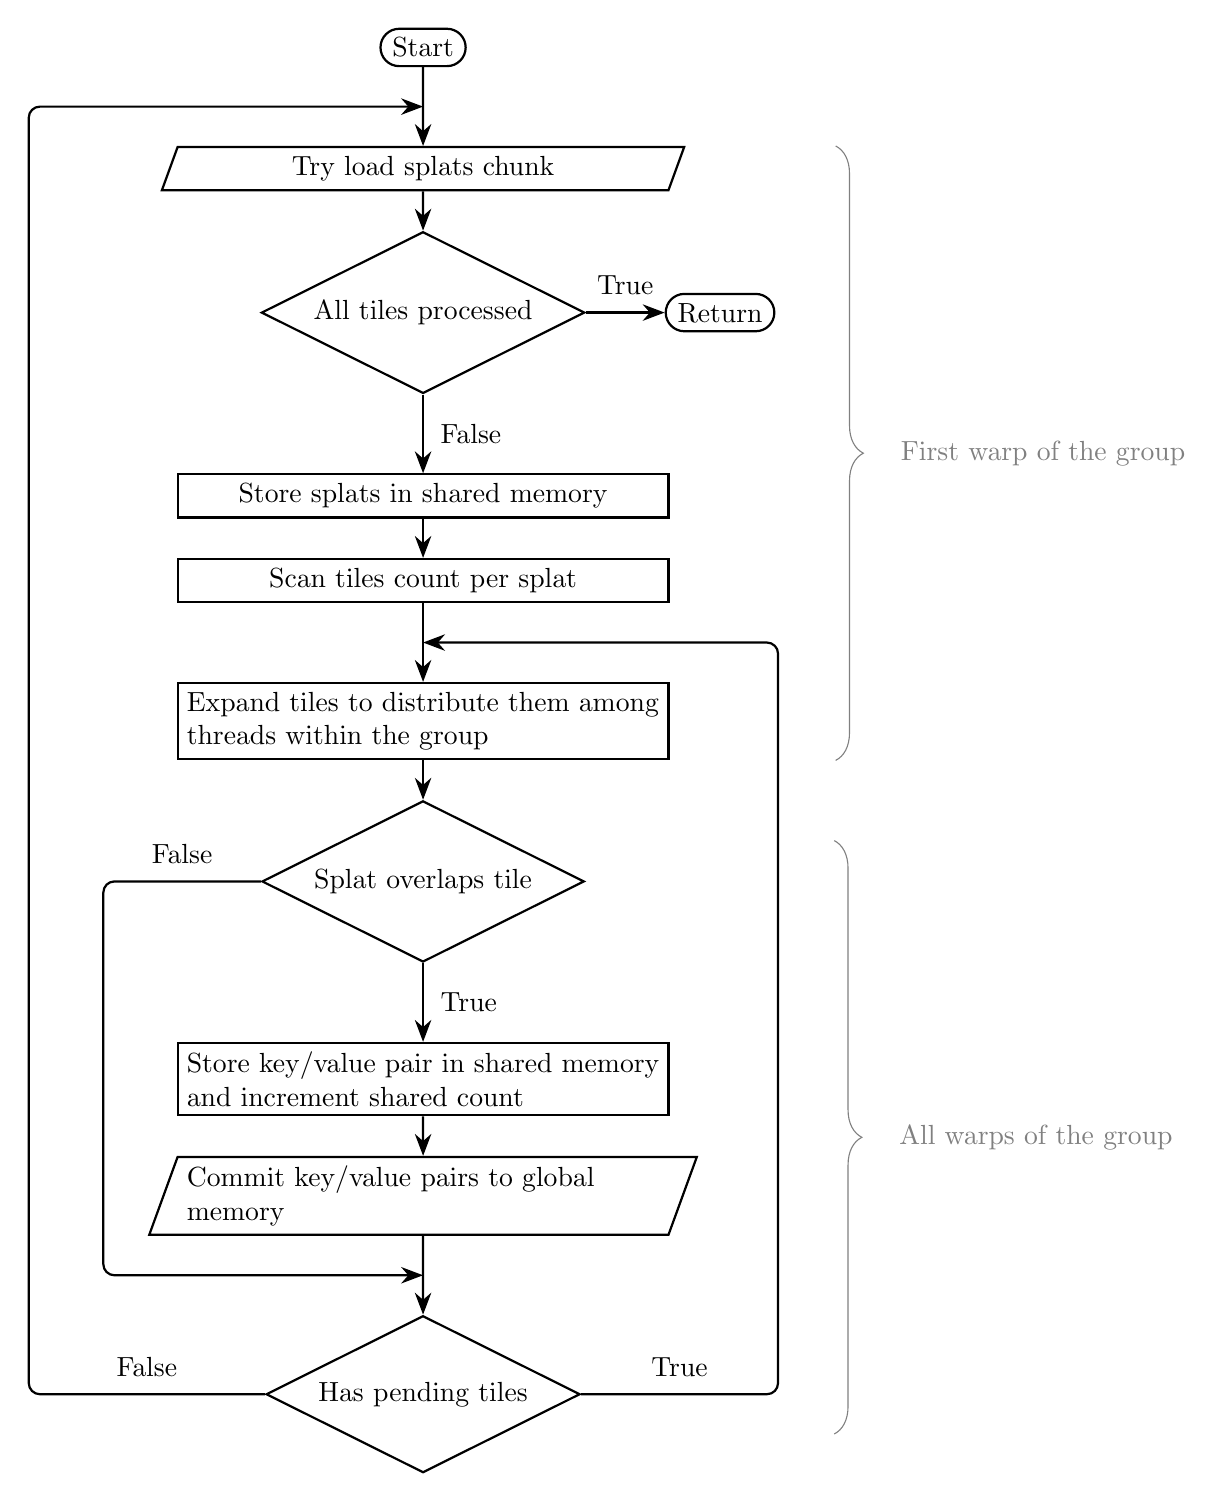
\begin{tikzpicture}
		\node (start) [startstop] {Start};
		\node (load-splats) [io,below=1.0 of start] {\textbox{Try load splats chunk}};
		\node (exit-if-empty) [decision,aspect=2,below=0.5 of load-splats] {All tiles processed};
		\node (return) [startstop,right=1 of exit-if-empty] {Return};
		\node (store-shared) [process,below=1.0 of exit-if-empty] {\textbox{Store splats in shared memory}};
		\node (scan) [process,below=0.5 of store-shared] {\textbox{Scan tiles count per splat}};
		\node (expand) [process,below=1.0 of scan] {\textbox{Expand tiles to distribute them among threads within the group}};
		%\node (overlap-test) [process,below=0.5 of expand] {\textbox{Each thread performs an ellipse/tile overlap test}};
		\node (write-if-overlap) [decision,aspect=2,below=0.5 of expand] {Splat overlaps tile};
		\node (write-shared) [process,below=1.0 of write-if-overlap] {\textbox{Store key/value pair in shared memory and increment shared count}};
		\node (write-global) [io,below=0.5 of write-shared] {\textbox{Commit key/value pairs to global memory}};
		\node (pending-tiles-test) [decision,aspect=2,below=1.0 of write-global] {Has pending tiles};
		
		\draw [arrow] (start) --  coordinate[midway](m1)(load-splats);
		\draw [arrow] (load-splats) -- (exit-if-empty);
		\draw [arrow] (exit-if-empty) -- coordinate[midway](m4)(store-shared);
		\draw [arrow] (exit-if-empty) -- coordinate[midway](m5)(return);
		\draw [arrow] (store-shared) -- (scan);
		\draw [arrow] (scan) -- coordinate[midway](m3)(expand);
		\draw [arrow] (expand) -- (write-if-overlap);
		\draw [arrow] (write-if-overlap) -- coordinate[midway](m6)(write-shared);
		\draw [arrow] (write-shared) -- (write-global);
		\draw [arrow] (write-global) -- coordinate[midway](m2)(pending-tiles-test);
		
		\draw [arrow] (write-if-overlap.west) -- coordinate[midway](m7) + (-2.0,0) |- (m2);
		\draw [arrow] (pending-tiles-test.west) -- coordinate[midway](m8) + (-3.0,0) |- (m1);
		\draw [arrow] (pending-tiles-test.east) -- coordinate[midway](m9) + (2.5,0) |- (m3);
		
		\node [black,right=0.1 of m4] {False};
		\node [black,above=0.1 of m5] {True};
		\node [black,right=0.1 of m6] {True};
		\node [black,above=0.1 of m7] {False};
		\node [black,above=0.1 of m8] {False};
		\node [black,above=0.1 of m9] {True};
		
		\draw [gray, decorate,decoration={brace, raise=6.0em, amplitude=1.0em}] 
		let \p1=(load-splats.north east) in (\x1,\y1)
		let \p2=(expand.south east) in (\x2,\y2)
		 (\x2,\y1) -- (\x2,\y2) node[pos=0.5,right=8.0em,gray]{First warp of the group};
		 
		\draw [gray, decorate,decoration={brace, raise=12.0em, amplitude=1.0em}] 
		let \p1=(write-if-overlap.north east) in (\x1,\y1)
		let \p2=(pending-tiles-test.south east) in (\x2,\y2)
		(\x2,\y1) -- (\x2,\y2) node[pos=0.5,right=14.0em,gray]{All warps of the group};
	
	\end{tikzpicture}
\end{document}